\documentclass[12pt]{article}
\usepackage[margin=1in]{geometry}
\usepackage[pdftex]{graphicx}
\usepackage{multirow}
\usepackage{setspace}
\usepackage{enumitem}
\pagestyle{plain}

\begin{document}

\noindent
% Course information
\begin{tabular*}{\textwidth}{l @{\extracolsep{\fill}} r}
  & \multirow{3}{*}{
\includegraphics[height=1.0in]{logo.jpg}} \\
  \large Particle Physics & \\
  \large Winter Quarter 2025 & \\
  \large Physics 130A & \\
\end{tabular*}
\vspace{10mm}

\noindent
% Professor information
\begin{tabular}{ l l }
  \multirow{6}{*}{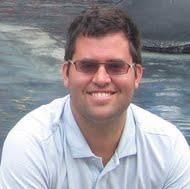
\includegraphics[height=1.25in]{mike.jpg}} & \\
  & \\
  & Michael Mulhearn \\
  & mulhearn@physics.ucdavis.edu \\
  & Physics 317 \\
  & \\
\end{tabular}
\vskip 0.5cm

\noindent
\begin{tabbing}
\hspace*{8em} \= \kill 
\textbf {Lecture:} \> M,W,F 9:00-9:50 AM in Lecture Teaching and Learning Complex 3210 (next to Silo, to the west) 
\end{tabbing}
\noindent
\begin{tabbing}
\hspace*{8em} \= \kill 
\textbf{Textbooks:} \> G: Introduction to Elementary Particles (2nd), Griffiths.\\
\> LN: Lecture Notes (Course website)\\
\> T: Modern Particle Physics, Thomson. (Optional)\\
\> An Introduction to Tensors and Group Theory for Physicists, Jeevanjee. (Optional)\\
\> (Jeevanjee is available online at the library)\\
\end{tabbing}
\noindent
\begin{tabbing}
\hspace*{8em}\= \hspace*{10em} \= \kill 
\textbf{Course TAs:} \> (TBD)
\end{tabbing}
\noindent
\begin{tabbing}
\hspace*{8em}\= \hspace*{10em} \= \kill 
\textbf{Office Hours:}
    \> Mulhearn: \> (TBD)
\end{tabbing}
\noindent
\begin{tabbing}
\hspace*{12em}\= \kill 
\textbf{Homework:} \> From 5-10 homework problem sets.\\
\textbf{Midterm Exams:} \> Two In-Class Midterms\\
\textbf{Final Exam:} \>  March, 21 2025 10:30 AM\\
\end{tabbing}
\noindent
\textbf {Course Description:}\\
Properties and classification of elementary particles and their
interactions. Experimental techniques. Conservation laws and
symmetries. Strong, electromagnetic, and weak
interactions. Introduction to Feynman calculus.\\[3pt]

\newpage

\noindent
\textbf{Reading:}\\ This course will be focused on Griffiths, and the
lecture notes, which draw from Thomson and Jeevanjee.  {\bf You are
  expected to read Giffiths chapters one and two on your own.}  That
material is accessible and will be tested through multiple choice
questions on the first midterm.\\[3pt]

\noindent
\textbf{Homework:}\\ There will be 5-10 homework assignments, which
you will submit to gradescope.  You may consult with other students
but your submitted work must be your own.  Your homework will be
graded on (sincere) effort only.  Homework will be a mixture of
excellent problems from Griffiths and some custom problems designed
to prepare you for the exams.  The grading scheme for the course
assumes students will be near $100\%$ on homework.  One late homework may
be submitted at (or before) the final exam for full credit.\\[3pt]

\noindent
\textbf{Exams:}\\ Exams will be in class, paper and pen or pencil
only, with no equation sheet, no internet, and no calculators.  The
exam will start with a quick answer, multiple choice part.  After
submitting that portion, you will pick up the second half of the exam,
consisting of longer problems with some equations provided.  No
practice exams will be provided.  Working through the homework
problems for yourself will be best preparation for the exams.  Timing
and scope of the exams will be finalized during the quarter.\\[3pt]

\noindent
\textbf {Grades:}\\ Final grades will be a mixture of homework and
exams.  The weighting will be adjusted to avoid the need for a curve.
It is assumed that your homework scores (graded on effort only) will
be near $100\%$.\\

\newpage

\noindent
\textbf {Course Schedule:}\\
This is a preliminary schedule which will evolve as the course
progresses.\\ You are expected to read and comprehend Griffith's
Chapters 1 and 2 on your own, and that material will be included on
the exams.\\[3pt]

\noindent
\begin{tabular}{llll}
\textbf{Week} & \textbf{Dates} & \textbf{Topics} & \textbf{Reading} \\
\hline
1  & Jan 6,8,10      & Vectors and Tensors      & LN Relativity \\
   &                 & Special Relativity       &               \\
\hline
2  & Jan 13,15,17    & Relativistic Kinematics  &  G 3.1-3.5    \\
\hline
3  & Jan 22,24       & Decay Rates and Cross Sections  & G: 6.1-6.2 \\
   &                 &                                 & TH: 3.1-3.5 \\
\hline
4  & Jan 27,29,31    & Feynman Calculus                & G: 6.3 \\
\hline
5  & Feb 3,5,7       & Symmetry and Spin               & TBD \\
\hline
6  & Feb 10,12,14    & Dirac Equation                 & G:7.1 \\
   &                 & Quantum Electrodynamics        & G:7.2-7.3 \\
\hline
7  & Feb 19,21       & Quantum Electrodynamcs         & G: 7.4-7.9    \\
\hline
8  & Feb 24,26,28    & Quantum Chromodynamics & TBD \\
\hline
9  & Mar 3,5,7       & TBD & \\
\hline
10 & Mar 10,12,14    & TBD & \\
\hline
\end{tabular}\\ \vskip 1cm

\end{document}

